\documentclass[12pt, a4paper]{article}

\usepackage{fontspec}
\usepackage{Alegreya}
\usepackage{polyglossia}
\usepackage{geometry}
\usepackage{amsmath, amssymb}
\usepackage{graphicx}
\usepackage{listings}
\usepackage[colorlinks, urlcolor=blue, linkcolor=black]{hyperref}
\usepackage{titling}
\usepackage{enumitem}
\usepackage{booktabs, longtable, ltablex}
\usepackage{calc}

\setmainlanguage{ukrainian}

\geometry{left=2cm, right=2cm, top=2.5cm, bottom=3cm}

\setlength{\parindent}{1.25cm}
\setlength{\parskip}{0pt}
\setcounter{secnumdepth}{3}

\setlist{topsep=0pt,partopsep=0pt}

\usepackage{xcolor}
\definecolor{codegray}{rgb}{0.5,0.5,0.5}
\definecolor{backcolour}{rgb}{0.95,0.95,0.95}
\lstdefinestyle{mystyle}{
    backgroundcolor=\color{backcolour},
    commentstyle=\color{codegray},
    keywordstyle=\color{black}\bfseries,
    numberstyle=\tiny\color{codegray},
    stringstyle=\color{purple},
    basicstyle=\ttfamily\footnotesize,
    breaklines=true,
    captionpos=b,
    keepspaces=true,
    numbers=left,
    numbersep=5pt,
    showspaces=false,
    showstringspaces=false,
}
\lstset{style=mystyle}

\title{Eat, Cry, Repeat}
\author{}
\date{}

\providecommand{\tightlist}{\setlength{\itemsep}{0pt}\setlength{\parskip}{0pt}}

\begin{document}

\begin{titlepage}
    \begin{center}
		{\Large
			МІНІСТЕРСТВО ОСВІТИ ТА НАУКИ УКРАЇНИ

			НАЦІОНАЛЬНИЙ ТЕХНІЧНИЙ УНІВЕРСИТЕТ УКРАЇНИ
			«КИЇВСЬКИЙ ПОЛІТЕХНІЧНИЙ ІНСТИТУТ ІМЕНІ ІГОРЯ СІКОРСЬКОГО»

			ФАКУЛЬТЕТ ІНФОРМАТИКИ ТА ОБЧИСЛЮВАЛЬНОЇ ТЕХНІКИ

			КАФЕДРА ІНФОРМАЦІЙНИХ СИСТЕМ ТА ТЕХНОЛОГІЙ
		}


		\vspace{60mm}
		{\large
			\textbf{ЗВІТ}

			\vspace{5mm}

			\textbf{До лабораторної роботи №2}

			\vspace{5mm}

			з дисципліни «Проектування Програмного Забезпечення»
		}

    \vspace{10mm}
    {\huge \textbf{Проект: "Eat, Cry, Repeat"}}

	\end{center}

	\vfill
    	\begin{minipage}[t]{0.30\textwidth}
		\textbf{Перевірив:}

		ст. викладач
	\end{minipage}
	\hfill
    	\begin{minipage}[t]{0.35\textwidth}
		\textbf{Виконали:}
	\end{minipage}

	\vfill

	\begin{center}
		{\bf
			Київ

			КПІ Ім. Ігоря Сікорського

			2025
		}
	\end{center}
\end{titlepage}

\renewcommand{\contentsname}{Зміст}
\tableofcontents
\newpage

\section{Вибір архітектурного підходу}

Для проекту "Eat, Cry, Repeat" було обрано \textbf{монолітну архітектуру}. Цей
підхід передбачає розробку системи як єдиного, цілісного додатку, де всі
компоненти (інтерфейс користувача, бізнес-логіка, доступ до даних) розгорнуті
як один сервіс.

\subsection{Обґрунтування вибору}

Вибір монолітної архітектури обґрунтований наступними факторами, що випливають
з вимог проекту:

\begin{itemize}
    \item Простота розробки та розгортання. На початковому етапі проекту, коли
        команда невелика, а функціонал чітко визначений, моноліт значно спрощує
        процес розробки. Немає потреби налаштовувати складну взаємодію між
        сервісами, керувати мережевими затримками чи розподіленими
        транзакціями. Розгортання зводиться до деплою одного застосунку, що
        ідеально відповідає стеку (FastAPI, Docker, Hetzner).

    \item Швидкість виходу на ринок (MVP). Мета першого етапу — швидко
        реалізувати ключовий функціонал (ведення щоденника, AI-roast) та
        перевірити гіпотезу. Монолітна архітектура дозволяє уникнути надмірної
        інженерної складності (overhead), пов'язаної з мікросервісами, і
        зосередитись на реалізації бізнес-цілей.

    \item Продуктивність. Всі внутрішні виклики між компонентами (наприклад,
        між контролером та сервісом доступу до даних) відбуваються в межах
        одного процесу, що виключає мережеві затримки. Це важливо для
        дотримання нефункціональних вимог щодо швидкості відповіді системи.

    \item Відсутність потреби у незалежному масштабуванні. На даному етапі
        немає підстав вважати, що якась частина системи (наприклад, профіль
        користувача) буде навантажена в рази більше, ніж інша (наприклад,
        ведення щоденника). Тому переваги мікросервісів у точковому
        масштабуванні не є критичними.
\end{itemize}

Таким чином, для стартапу "Eat, Cry, Repeat" монолітна архітектура є найбільш
раціональним та ефективним рішенням, що дозволяє швидко та з меншими витратами
досягти поставлених цілей.

\section{Створення високорівневої архітектури}

Для візуалізації високорівневої архітектури було використано модель C4, яка
дозволяє описати систему на різних рівнях абстракції. Це допомагає зрозуміти її
структуру як з точки зору бізнесу, так і з технічної перспективи.

\subsection{Діаграма контексту системи (C4 Level 1)}

Ця діаграма (Рис. \ref{fig:c4_context}) показує систему "Eat, Cry, Repeat" як
"чорну скриньку" в її оточенні. Вона ілюструє основних акторів, які взаємодіють
із системою, та зовнішні залежності.

\begin{figure}[h!]
    \centering
    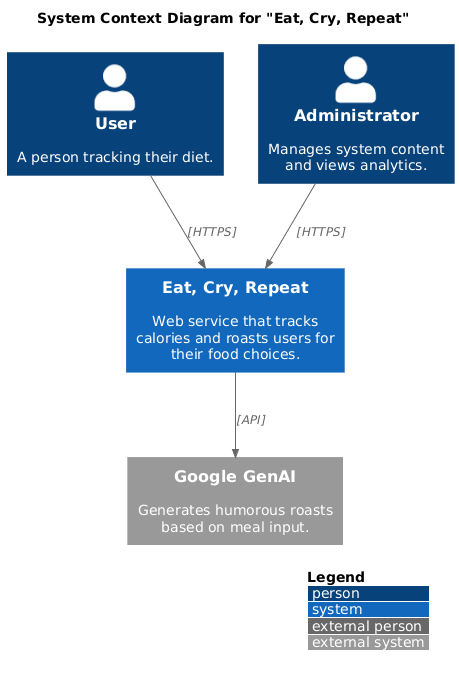
\includegraphics[width=0.9\textwidth]{c4_context.png}
    \caption{Діаграма контексту системи "Eat, Cry, Repeat"}
    \label{fig:c4_context}
\end{figure}

\textbf{Актори:}
\begin{itemize}
    \item Користувач (User): Основний споживач сервісу, який веде щоденник
        харчування.

    \item Адміністратор (Admin): Роль для керування системою, наприклад, базою
        продуктів.
\end{itemize}

\textbf{Зовнішні системи:}
\begin{itemize}
    \item Google GenAI: Зовнішній сервіс штучного інтелекту, що
        використовується для генерації гумористичних коментарів ("roasts").
\end{itemize}

\subsection{Діаграма контейнерів (C4 Level 2)}

Діаграма контейнерів (Рис. \ref{fig:c4_container}) "заглядає всередину" системи
і показує її основні розгортаємі частини (контейнери).

\begin{figure}[h!]
    \centering
    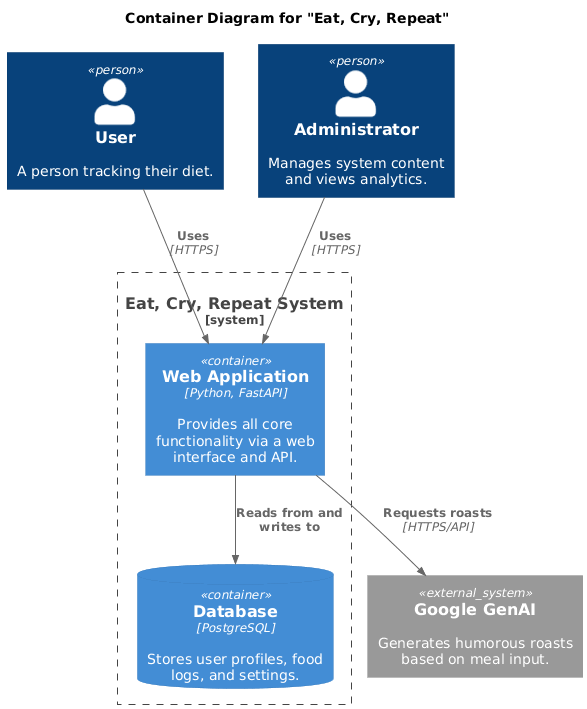
\includegraphics[width=0.9\textwidth]{c4_container.png}
    \caption{Діаграма контейнерів}
    \label{fig:c4_container}
\end{figure}

Система складається з двох основних контейнерів:
\begin{itemize}
    \item Веб-додаток (Web Application): Монолітний бекенд, розроблений на
        Python з використанням фреймворку FastAPI. Він реалізує всю
        бізнес-логіку, обробляє API-запити, взаємодіє з базою даних та
        зовнішнім AI-сервісом.
    \item База даних (Database): Сховище даних на основі PostgreSQL. Тут
        зберігається вся інформація про користувачів, їх профілі, щоденники
        харчування та налаштування.
\end{itemize}

\subsection{Діаграма компонентів (C4 Level 3)}

Ця діаграма (Рис. \ref{fig:c4_component}) деталізує внутрішню структуру
контейнера "Веб-додаток", показуючи його основні логічні модулі (компоненти) та
їх взаємодію.

\begin{figure}[h!]
    \centering
    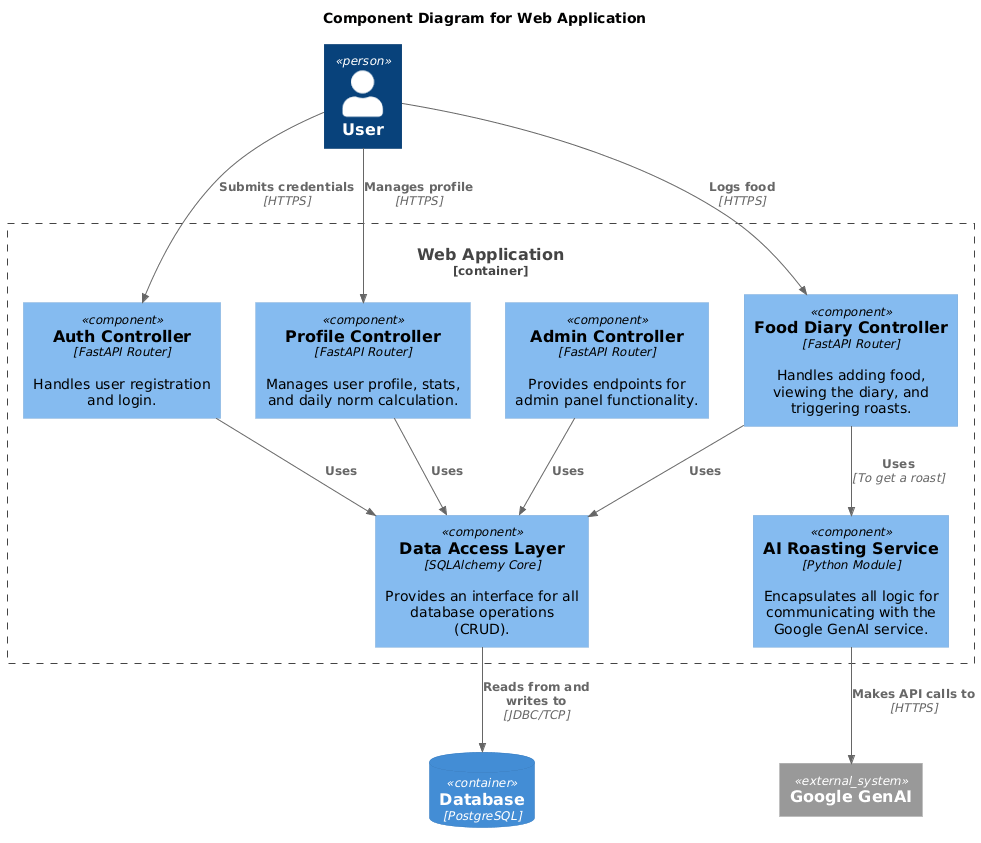
\includegraphics[width=\textwidth]{c4_component.png}
    \caption{Діаграма компонентів веб-додатку}
    \label{fig:c4_component}
\end{figure}

Основні компоненти:
\begin{itemize}
    \item Контролери (Controllers): Обробляють вхідні HTTP-запити. Розділені за
        функціональністю: автентифікація, профіль, щоденник, панель
        адміністратора.

    \item Сервіс AI Roasting (AI Roasting Service): Інкапсулює логіку взаємодії
        із зовнішнім сервісом Google GenAI.

    \item Шар доступу до даних (Data Access Layer): Відповідає за всі операції
        з базою даних, абстрагуючи логіку роботи з SQL.
\end{itemize}

\section{Деталізоване проектування компонентів}

Для деталізації ключових аспектів системи було обрано дві UML-діаграми:
діаграму варіантів використання та діаграму послідовності.

\subsection{Діаграма варіантів використання (Use Case Diagram)}

\subsubsection{Обґрунтування вибору}
Діаграма варіантів використання є ідеальним інструментом для візуалізації
функціональних вимог до системи з точки зору користувача. Вона відповідає на
питання "Що система може робити для користувача?". Ця діаграма допомагає чітко
визначити межі системи та основні сценарії взаємодії, що є критично важливим на
етапі проектування для узгодження бачення продукту між усіма членами команди.

\subsubsection{Опис діаграми}
Діаграма (Рис. \ref{fig:use_case}) показує двох акторів та їх основні
можливості в системі.

\begin{figure}[h!]
    \centering
    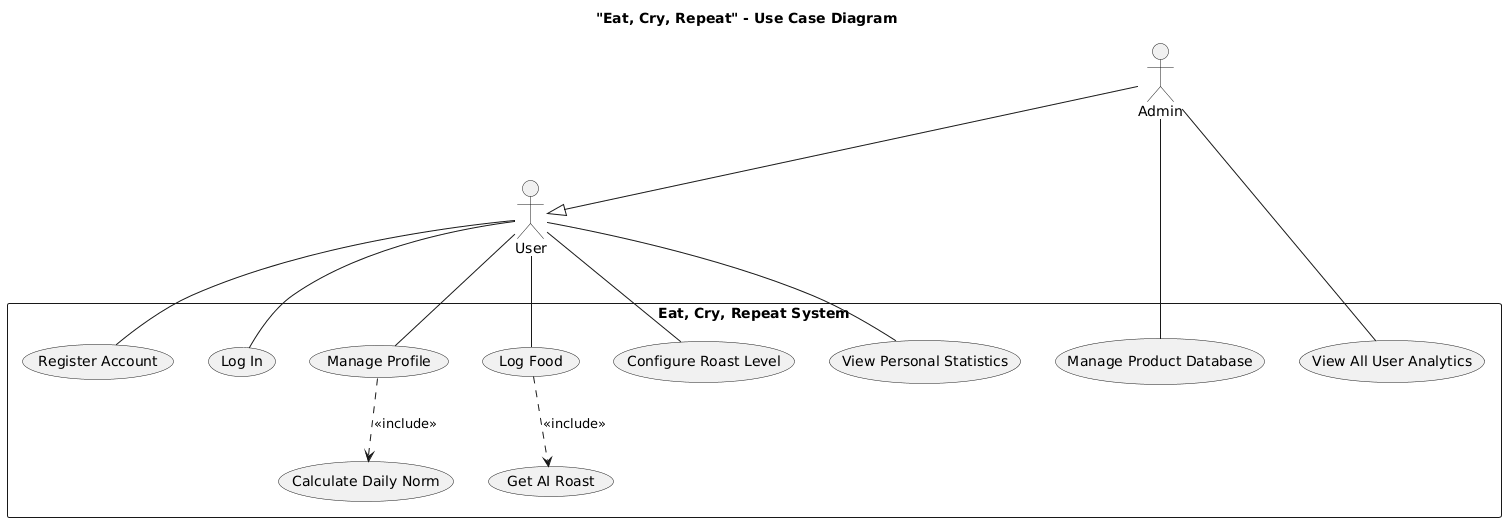
\includegraphics[width=\textwidth]{use_case.png}
    \caption{Діаграма варіантів використання}
    \label{fig:use_case}
\end{figure}

\textbf{Користувач (User)} може:
\begin{itemize}
    \item Реєструватися та входити в систему.
    \item Керувати своїм профілем (вводити параметри, на основі яких
        розраховується добова норма калорій).
    \item Вести щоденник харчування (додавати їжу).
    \item Налаштовувати рівень "roast" від AI-асистента.
    \item Переглядати статистику.
\end{itemize}
Ключова взаємодія — \textbf{Log Food} — автоматично включає функцію \textbf{Get
AI Roast}, що підкреслює унікальність додатку.

\subsection{Діаграма послідовності (Sequence Diagram)}

\subsubsection{Обґрунтування вибору}
Якщо діаграма варіантів використання показує \textit{що} система робить, то
діаграма послідовності показує \textit{як} вона це робить. Для деталізації було
обрано найважливіший бізнес-процес — додавання їжі та отримання коментаря від
AI. Ця діаграма демонструє динамічну взаємодію між компонентами системи в часі,
що дозволяє виявити потенційні вузькі місця та перевірити логіку
нефункціональних вимог (наприклад, час відповіді AI).

\subsubsection{Опис діаграми}
Діаграма (Рис. \ref{fig:sequence_roast}) ілюструє покрокову взаємодію при
додаванні користувачем нового запису до щоденника.

\begin{figure}[h!]
    \centering
    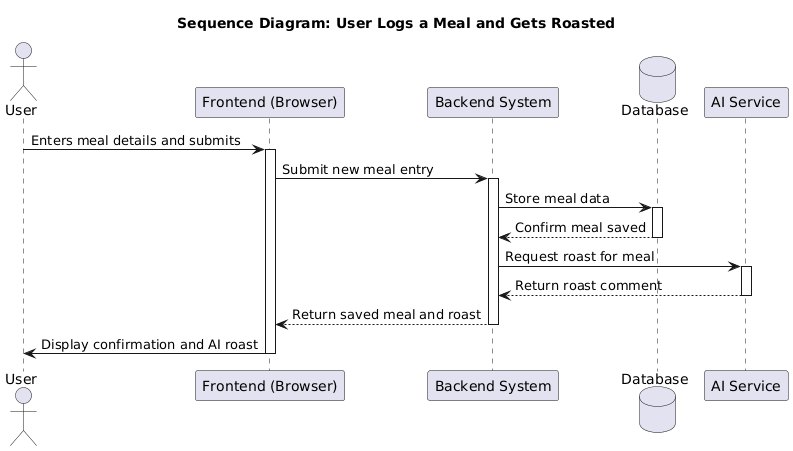
\includegraphics[width=\textwidth]{sequence_roast.png}
    \caption{Діаграма послідовності: Додавання їжі та отримання "roast"}
    \label{fig:sequence_roast}
\end{figure}

Процес виглядає наступним чином:
\begin{enumerate}
    \item Користувач через фронтенд надсилає дані про спожиту їжу.
    \item Фронтенд робить запит до бекенду.
    \item Бекенд зберігає інформацію про їжу в базу даних.
    \item Після успішного збереження бекенд звертається до зовнішнього
        AI-сервісу для генерації коментаря.
    \item AI-сервіс повертає згенерований текст.
    \item Бекенд надсилає фронтенду підтвердження про збереження та отриманий
        коментар.
    \item Фронтенд відображає результат користувачеві.
\end{enumerate}

\section{Висновок}

У ході виконання лабораторної роботи було спроектовано архітектуру програмного
забезпечення для веб-сервісу "Eat, Cry, Repeat".

Було обрано та обґрунтовано \textbf{монолітну архітектуру} як оптимальну для
поточного етапу розвитку проекту, що дозволить швидко розробити та запустити
MVP.

За допомогою \textbf{моделі C4} було створено багаторівневий опис архітектури,
що включає діаграми контексту, контейнерів та компонентів. Це забезпечує чітке
розуміння системи на різних рівнях деталізації.

Для детального проектування було використано \textbf{UML-діаграми}:
\begin{itemize}
    \item Діаграма варіантів використання для визначення
        функціонального обсягу системи.
    \item Діаграма послідовності для моделювання динамічної поведінки ключового
        бізнес-процесу.
\end{itemize}

Розроблена архітектура є логічною, відповідає функціональним та
нефункціональним вимогам, і створює надійний фундамент для подальшої розробки
програмного продукту.

\end{document}
